\chapter{Personal Reflection} % Main chapter title

\label{Chapter4} % Change X to a consecutive number; for referencing this chapter elsewhere, use \ref{ChapterX4}

\lhead{Chapter 4. \emph{Personal Reflection}} % Change X to a consecutive number; this is for the header on each page - perhaps a shortened title


My initial draft of this chapter was written in a chronological fashion, discussing and reflecting on my academic and professional experience year by year.
I, however, discovered some recurring themes (e.g. problems regarding my time management) which were difficult to fully reflect on when the evidence/ relevant discussion points were scattered throughout my years at Heriot-Watt University.
I have therefore decided to structure this chapter by themes, so that I can efficiently reflect on my progress/ growth in different areas from the start to the end of my degree.
\hl{The themes I will be reflecting on are: ...}


%----------------------------------------------------------------------------------------
%	SECTION X
%----------------------------------------------------------------------------------------

\section{Professionalism}

\begin{comment}
A professional is someone that:
\begin{itemize}
    \item Applies their body of knowledge with rigorous standards of skill, care and diligence,
    \item Seeks continuously to maintain up to date \& to improve knowledge \& skills in themselves and others,
    \item Is entirely trustworthy, ethical and acts with integrity.
    \item Fulfils an overriding duty to society/mankind and thereafter the client 
    \item Treats all people fairly \& with respect 
\end{itemize}
\end{comment}

Points to discuss:
\begin{itemize}
    \item log (and then asked for it, glad on reflection for my initiative/ proactiveness);
    \item needing to be opportunistic rather than strategic to see Sandy (stats on number of meetings...);
    \item Applies their body of knowledge with rigorous standards of skill, care and diligence;
    \item personal project and carrying out a personal programme of work (G3);
    \item compilation of work produced.
    \item Giving them what they needed, not what they asked for (e.g. quiz initiative + full development)
    \item adapting to their way of working while maintaining productivity...
\end{itemize}


\subsection{Log Keeping}

During my first placement at Hultin \& Lundquist Arkitekter in 2013, I was asked to keep a timesheet which I was to submit on a monthly basis.
As I was getting paid an hourly rate, my salary was calculated from that timesheet.
This experience kick-started my habit of keeping a time log during my following placements because it made me think of it as a fundamental professional \hl{expectation/ obligation/ responsibility}.

When I started my placement at Arup in 2016, I knew from reading my contract that the company expected me to submit a report about my placement by the end of it.
I therefore kept a daily diary where I jotted down notes about the work I had done and the things I had learned in addition to recording the hours I worked.
This not only facilitated the writing of the report, but also helped me monitor the progress of my tasks and strengthen my knowledge acquisition.
On the one hand, keeping a record of my time and activities helped me monitor my progress and ensure that the rate I was working at was good enough.
Unlike university, there is not much structure to working in industry: there are no numbered weeks or semesters, and there are not always deadlines etc.
Within this chaotic environment, the time/ activity log provided me with quantitative information of my rates of progress, allowing me to structure my time better.
On the other hand, keeping a record of the things I learned strengthened my knowledge acquisition for a few reasons:
\begin{itemize}
	\item I found myself frequently revisiting and implementing my little ``lesson" notes in order to carry out my design tasks at Arup.
	\item Some notes provided me with a practical understanding and knowledge foundation for some of my future courses at Heriot-Watt University, such as \textit{Electrical \& Lighting Services for Buildings}.
	In this example, I had learned a rule for sizing cables at Arup, which is represented by Equation \ref{eqn:GoldenRule} and Figure \ref{fig:GoldenRule}\footnote{
		$I_b$ is the design current, $I_n$ is the protective device rating, and $I_z$ is the cable current capacity.
		$I_b$ should not be greater than $I_n$, or else it would trip the protective device.
		$I_n$ should not be greater than $I_z$, or else the cable might catch on fire when the current is greater than the cable's capacity.
		$I_z$ should not be smaller than $I_b$, or else the load would not get the required current to operate.
		}.
	When we were then taught how to size cables in class, I realised that I was able to better understand the lesson due to my practical experience at Arup and the notes I had taken, which I was able to re-visit.
	
	\begin{equation}
	I_b \leq I_n \leq I_z
	\label{eqn:GoldenRule}
	\end{equation}
	
	\begin{figure}[H]
		\centering
		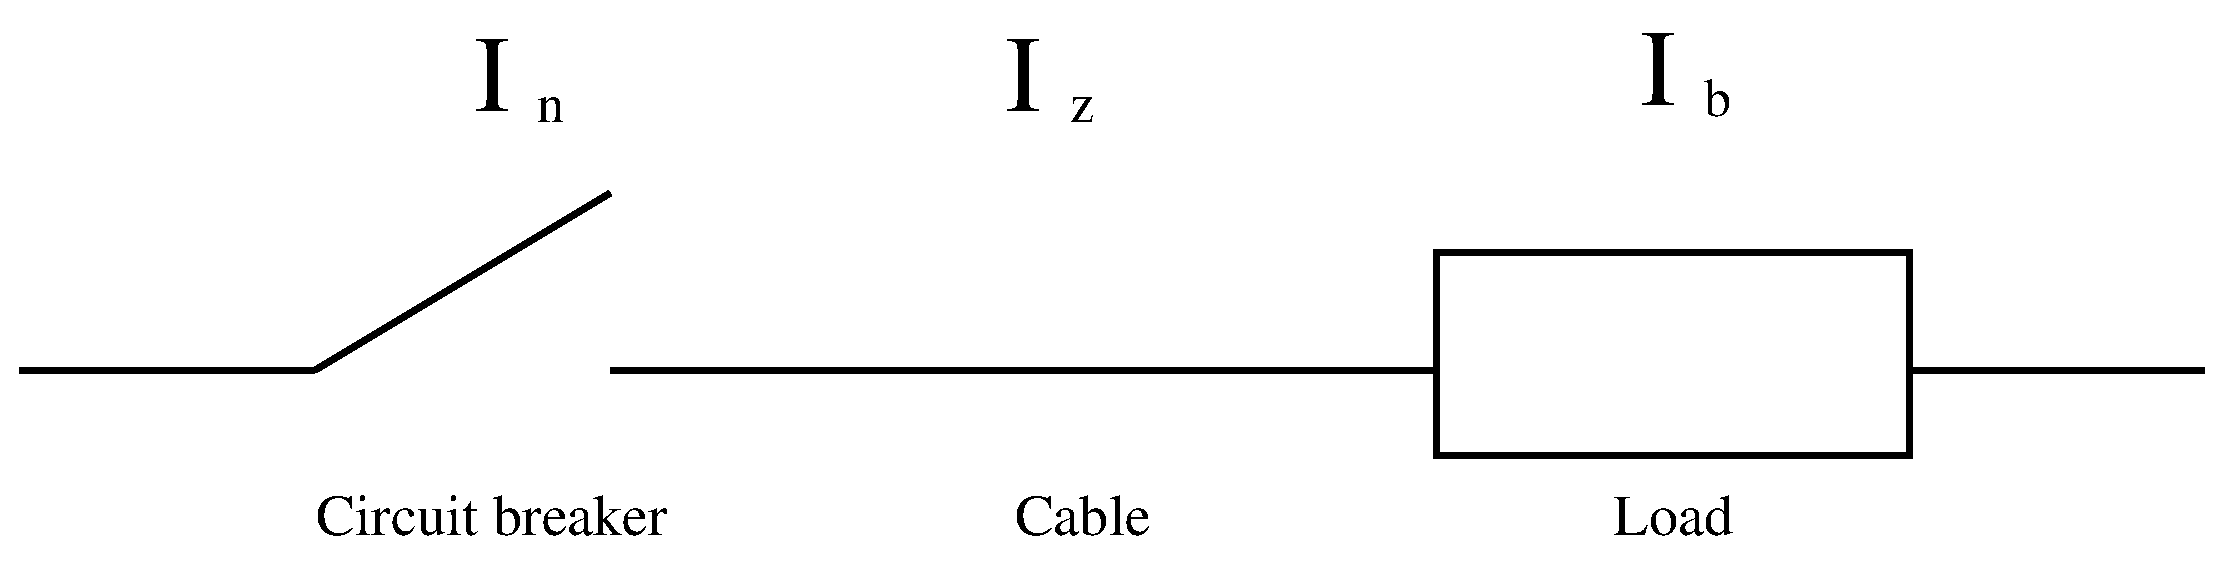
\includegraphics[width=10cm]{figures/GoldenRule.eps}
		\rule{10cm}{0.5pt} % use line???
		\caption{Graphical explanation for cable sizing.}
		\label{fig:GoldenRule}
	\end{figure}
	
	\item The simple act of writing down a new piece of information helps me to retain that knowledge better.
\end{itemize}



From these experiences, I developed a habit of keeping a time/ activity/ lesson log at my following placements for my own benefit but also in case my employers required me to submit a timesheet.
Sometimes this was the case (e.g. at Hoare Lea and Sunamp), and other times it was not (e.g. at Sweco).
A month into my placement at Sunamp, for example, I was asked to submit a timesheet.
On reflection, I am glad for my proactivity in keeping a log at Sunamp since they did not inform me on the timesheet requirement at the start of my placement.







%----------------------------------------------------------------------------------------
%	SECTION X
%----------------------------------------------------------------------------------------
\newpage
\section{Academic Performance}



%----------------------------------------------------------------------------------------
%	SECTION X
%----------------------------------------------------------------------------------------

\section{Perfectionism vs. Time Management}



%----------------------------------------------------------------------------------------
%	SECTION X
%----------------------------------------------------------------------------------------

\section{Future Learning and Career Aspirations}